% =============================================================================
% CW short methods paper — arXiv stat.ME (cross-list stat.AP)
% Prose draft 2026-08-25 (v2) from drafts/PAPER_SKELETON.md.
% All numbers are LOCKED from simulation/SIM1B_RESULTS.md and toy/out/.
% Do NOT alter numbers without rerunning simulation/sim1_engine.R.
% Build: /Library/TeX/texbin/pdflatex main (twice)
% =============================================================================
\documentclass[11pt]{article}
\usepackage[margin=1.1in]{geometry}
\usepackage{amsmath,amssymb}
\usepackage{graphicx}
\usepackage{booktabs}
\usepackage{subcaption}
\captionsetup{font=footnotesize}   % captions two steps below the 11pt body
\usepackage{placeins}       % \FloatBarrier: keep results figures inside Results
\usepackage[round]{natbib}
\usepackage[colorlinks=true,linkcolor=blue!50!black,citecolor=blue!50!black,urlcolor=blue!50!black]{hyperref}
\usepackage{xcolor}
\newcommand{\todo}[1]{\textcolor{red!70!black}{[TODO: #1]}}
\newcommand{\Obar}{\bar{O}}
\newcommand{\wstar}{w^{*}}

\title{Carrier-Weighted Networks: Separating Coherent Minority Structure
from Incoherent Edges with Matched Pooled Correlations}
% PI DECISION 1 resolved 2026-08-26: sole author, name/affiliation as in
% JAMA Netw Open 2024;7(7):e2420934 (doi:10.1001/jamanetworkopen.2024.20934)
\author{Yong-Wook Shin\\[2pt]
\normalsize Department of Psychiatry, Asan Medical Centre,\\
\normalsize University of Ulsan College of Medicine, Seoul, Korea\\
\normalsize \texttt{shaman\_korea@mac.com}}
\date{\today}

\begin{document}
\maketitle

\begin{abstract}
In networks built from questionnaire data, a pooled edge correlation ---
the correlation of one item pair --- is an average over respondents: the
same value can arise from weak coupling in everyone, strong coupling in a
coherent minority, or accidental co-endorsement by scattered, mutually
unrelated subsets. Pooled network pipelines cannot tell these apart. We
introduce an edge-level estimator of carrier coherence that requires no
prespecified respondent groups,
$\wstar_e=|\rho_e|(1-G_e)\max(\Obar_e,0)$: the product of the pooled
correlation magnitude $|\rho_e|$, an evenness-of-support factor $(1-G_e)$,
and a coherence factor $\max(\Obar_e,0)$ measuring whether the respondents
who carry an edge also carry the neighbouring edges that share an item with
it. In a preregistered simulation with pooled
correlations matched by calibrated design, the estimator separated
minority-carried community edges from planted incoherent edges
(``distractors'') with an area
under the receiver operating characteristic curve (AUROC) of
$.985$ versus $.469$ for raw correlations (paired difference $+.516$,
$95\%$ confidence interval $[+.506,+.526]$). A concentration-only
variant of the estimator remained at chance while a coherence-only variant
matched the full estimator --- the separation is due to the coherence
factor alone. Community recovery by the full pipeline showed no
improvement at $n=600$: by design, both pipelines drew their candidate
edges from the same raw-correlation filter, so reweighting could not
restore true edges that the selection step had already discarded.
\end{abstract}

% =============================================================================
\section{Introduction}\label{sec:intro}

A correlation between two questionnaire items is an average over respondents.
The estimate $|\rho|=.45$ is compatible with at least three different
data-generating stories: (a) a weak coupling present in essentially every
respondent; (b) a strong coupling present in a coherent $30\%$ minority and
absent elsewhere; and (c) no population-wide coupling at all, but incidental
co-endorsement by scattered subsets of respondents who have nothing else in
common. Standard psychometric network pipelines --- regularized partial
correlations or a maximally filtered graph, followed by community detection
\citep{epskamp2018,massara2016,pons2006,golino2017} --- operate entirely on
the pooled value and are therefore blind to the distinction. This is an
edge-level instance of the familiar warning that group-level statistics need
not describe any individual: the ecological fallacy in its psychometric form
\citep{molenaar2004,fisher2018}.

The blindness has two concrete costs. First, communities carried by a
coherent minority are attenuated at the pooling stage and are absorbed into
neighbouring communities or removed when the network is pruned to its
strongest edges (sparsification), because each of their edges looks
individually weak. Second, edges of type (c) --- pooled
correlations without any common set of respondents supplying them;
hereafter \emph{distractor} edges --- pass every pooled screen and
enter the network as if they were structure. Both errors leave no trace in
pooled fit statistics: the network that results is internally consistent and
wrong.

This paper contributes an edge-level estimator of carrier coherence that
requires no prespecified respondent groups. The estimator separates
coherent minority-carried structure from incoherent edges whose pooled
correlations match, and it can be incorporated into the standard bootstrap
exploratory graph analysis (bootEGA) pipeline by replacing the original
edge weights \citep{christensen2021}. Unlike mixture or
latent-class network models, it neither partitions respondents nor requires a
prespecified group-membership variable; the carriers of different edges may
overlap, nest, or cross-cut freely. It is also distinct from group-comparison
methods \citep{jamison2024} and meta-analytic techniques: the heterogeneity of
interest is between respondents within a single sample. The estimator changes
only the weights of edges retained by the pipeline's candidate-selection
step, leaving community detection and resampling-based inference to the
downstream pipeline.

% =============================================================================
\section{The carrier-weighted estimator}\label{sec:estimator}

\subsection{Setup and carrier profiles}
Let $x_{rj}\in\{0,1\}$ be the response of respondent $r$ to item $j$, and let
$\rho_e$ be the tetrachoric correlation for the item pair $e=(j,k)$. Define
the per-respondent contribution of respondent $r$ to edge $e$ as
\begin{equation}
S_{re} \;=\; (x_{rj}-\bar{x}_j)\,(x_{rk}-\bar{x}_k),
\end{equation}
the $r$-th summand of the covariance. The vector
$S_{\cdot e}=(S_{1e},\dots,S_{ne})$ is the \emph{carrier profile} of the
edge: it records who supplies the association. Because the summand is
centred, the profile is a signed contribution vector, not an endorsement
indicator: a respondent endorsing both items and a respondent endorsing
neither both contribute positively (the $(0,0)$ cell contributes
$\bar{x}_j\bar{x}_k$). ``Carrier'' is a mnemonic for the respondents whose
contributions dominate the positive mass of this vector; every quantity
below is computed from the full signed profile, never from a thresholded
carrier set. The estimator is deliberately hybrid in scale: the magnitude
factor uses the tetrachoric $\rho_e$ (latent scale), while the profile is
computed on the observed binary responses, where the respondent dimension
still exists. Pooling collapses this vector
to its mean; everything the present method does is done before that collapse.

\subsection{Two carrier components}
Two properties of the carrier profile carry the diagnostic information.

\emph{Concentration.} The Gini coefficient $G_e$ of the magnitudes
$|S_{re}|$\footnote{Computed in the standard sorted-index form: with
$v_{(1)}\le\dots\le v_{(n)}$ the sorted magnitudes $|S_{re}|$,
$G_e=2\sum_{r} r\,v_{(r)}\big/\big(n\sum_{r} v_{(r)}\big)-(n+1)/n$, with no
small-sample correction.} measures how unevenly the edge's support is
distributed over respondents. An edge carried by everyone has low $G_e$; an edge carried by a
small subset --- coherent or not --- has high $G_e$. The even-support factor
$(1-G_e)$ down-weights concentrated edges.

\emph{Coherence.} Let $\mathcal{N}(e)$ be the set of edges that share a node with
$e$ --- the neighbours of $e$ in the line graph of the network (the
derived graph whose nodes are the original network's edges). $\Obar_e$ is
the mean cosine between the carrier profile of $e$ and those of its
neighbours:
\begin{equation}
\Obar_e \;=\; \frac{1}{|\mathcal{N}(e)|}\sum_{f\in \mathcal{N}(e)}
\frac{\langle S_{\cdot e},\,S_{\cdot f}\rangle}
     {\lVert S_{\cdot e}\rVert\,\lVert S_{\cdot f}\rVert}.
\label{eq:obar}
\end{equation}
Only node-sharing pairs enter the average --- for $e=(j,k)$ that is
$\deg(j)+\deg(k)-2$ cosines, rather than a comparison of $e$ with all
$|E|-1$ other edges --- so the statistic is local and computationally
inexpensive even in dense networks; the structural reason
for this restriction is given in Section~\ref{sec:wedge}. $\Obar_e$ asks the
only question that concentration cannot: \emph{do the same respondents carry
the neighbouring edges?}

\subsection{Why neighbour alignment: the wedge --- a node-sharing edge
pair --- is the minimal detection unit}
\label{sec:wedge}
A single edge, considered alone, contains no information that discriminates
scenario (b) from scenario (c) of the Introduction. The pooled $\rho_e$ has
already collapsed the respondent dimension. Concentration does not help
either: a real minority-carried edge and an accidental co-endorsement are
\emph{both} concentrated, so $G_e$ assigns them similar values. This is the
a-priori reason to expect a concentration-only weighting to fail --- a
prediction the ablation in Section~\ref{sec:results} tests directly.

The discriminating evidence lives one level up. Latent factors load on
\emph{nodes} (items), not on edges. If a factor $F$ loads on item $j$, it
leaves its trace simultaneously on every edge through $j$ --- $(i,j)$,
$(j,k)$ --- and, crucially, that trace passes through the \emph{same}
respondents, namely those in whom $F$ is active. The shared node is the
conduit of the common cause. A distractor edge's carriers, by contrast, have
no structural reason to overlap with the carriers of any adjacent edge, so
its expected alignment is zero.

The minimal unit of factor detection is therefore not the edge but the
node-sharing edge pair --- the \emph{wedge}. Just as a correlation is a
two-node statistic, carrier coherence is a two-edge statistic, one order up:
$\Obar$ is a statistic on the line graph of the network, and the estimator's
essence is to lift inference from node pairs to edge pairs. A community, in
this view, is a connected set of high-coherence wedges sharing one latent
cause, and carrier alignment is the empirical fingerprint of that sharing.

\subsection{The full weight}
The estimator, locked in this form by the preregistration
(Section~\ref{sec:sim}), combines the pooled magnitude with both carrier
components:
\begin{equation}
\wstar_e \;=\; |\rho_e|\,(1-G_e)\,\max(\Obar_e,\,0).
\label{eq:cw}
\end{equation}
The positive-part rule --- a gate that removes edges with $\Obar_e<0$ ---
reflects a requirement of the downstream community-detection algorithm:
walktrap \citep{pons2006} interprets a positive weight as attraction, so an
edge whose carriers systematically \emph{oppose} those of its neighbours is
removed rather than passed through as a small positive weight.

\subsection{The minimal toy example: one triangle, two stories}\label{sec:toy}
If the wedge is the minimal detection unit, the natural worked example is
the smallest structure made entirely of wedges: the closed triangle on
three items $i,j,k$, whose three edges $(i,j)$, $(j,k)$, $(i,k)$ form
three node-sharing pairs, so that every edge's $\Obar$ is
the mean of its two wedge cosines. Closing the triangle also closes a
loophole a two-edge example leaves open: with an open wedge, the unused
third pair $(i,k)$ can still differ between scenarios, so a sceptic could
ask whether triadic closure alone --- the presence or absence of the third
edge completing the triangle --- would have separated them. Here it
cannot, by construction. Figure~\ref{fig:toy} shows two deterministic
scenarios on $n=18$ respondents (no random seed) in which \emph{every}
pooled $2\times2$ contingency table --- all three edges, both scenarios ---
has the same four cells. All pooled pairwise quantities are therefore
identical as a matter of arithmetic identity, not approximate matching:
every $\phi$ coefficient is $.25$, every tetrachoric correlation $.40$,
every Gini coefficient $.29$, and all item marginals coincide. Every $S_{re}$ entry is a multiple of $1/9$;
the whole example can be verified by hand in a few minutes.

In scenario A one minority (respondents 1--3) endorses all three items and
carries all three edges, while nine singleton respondents (three per item)
endorse one item each, filling the off-diagonal cells. All three carrier
cosines equal $+2/3$, so $\Obar=+2/3$ and every edge survives with
$\wstar=.19$. In scenario B the same pooled tables are produced by three
\emph{disjoint} minorities --- respondents 1--3 co-endorse $(i,j)$, 4--6
$(j,k)$, 7--9 $(i,k)$: every pairwise carrier cosine equals $-1/3$, so
$\Obar=-1/3$ and all three edges are removed. No pooled pairwise quantity
--- correlation, concentration, marginal, or any function of them,
including triadic closure --- distinguishes the panels; the eighteen
respondents do. (The full three-way $2\times2\times2$ table does differ, as
it must: A has three respondents in the $(1,1,1)$ cell, B has none. The
estimator recovers exactly this respondent-level information from pairwise
objects, without ever forming the higher-order table.) Note that scenario
B's edges are perfectly real \emph{within their own carriers} --- what the
carrier profiles withhold is evidence of a \emph{shared} cause, and that is
exactly the evidence the estimator weights. This point returns at scale as
the ground-truth (oracle) diagnostic of Section~\ref{sec:results}.

\begin{figure}[!htb]
\centering
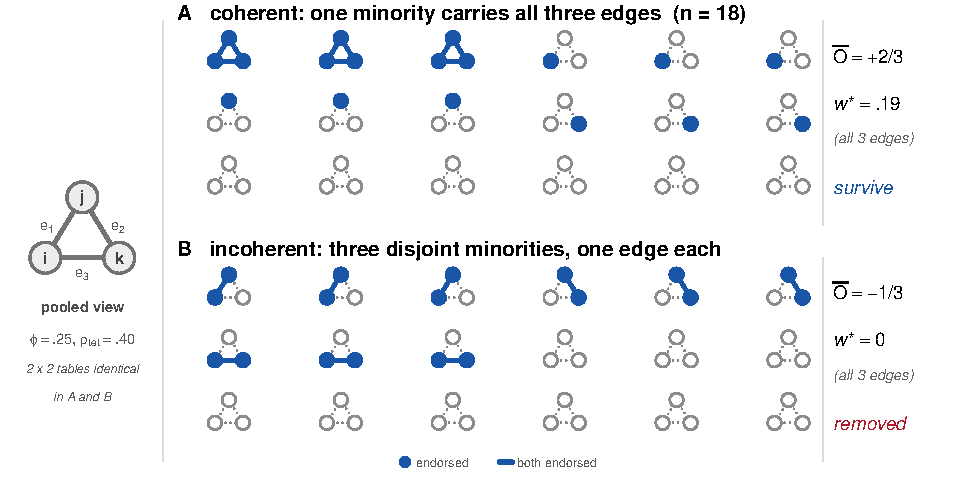
\includegraphics[width=.92\textwidth]{figs/fig1_triangle.pdf}
\caption{The minimal toy example: one closed triangle on items $i,j,k$,
$n=18$, two deterministic scenarios whose pooled $2\times2$ tables are
\emph{identical} on every edge (Section~\ref{sec:toy} gives the shared
values). Each respondent is drawn as their own copy of the triangle, its
outline dotted: filled nodes mark endorsed items; an edge is drawn solid
if and only if the respondent endorses both of its endpoints (the
respondent \emph{carries} that edge); the pooled view (left, drawn once)
is identical for the two scenarios. \textbf{A}: one minority carries all
three edges, all carrier cosines are $+2/3$, and every edge survives
($\wstar=.19$). \textbf{B}: three disjoint minorities carry one edge
each, all carrier cosines are $-1/3$, and the gate removes every edge. No
pooled pairwise statistic distinguishes the panels; the carrier profiles
do.}
\label{fig:toy}
\end{figure}

The estimator does not address cancellation across opposite-signed carrier
groups or within-person dynamics \citep{molenaar2004}; these limitations are
discussed in Section~\ref{sec:discussion}.

\FloatBarrier  % Figure 1 (toy) must stay inside Section 2, next to the toy example

% =============================================================================
\section{Preregistered simulation}\label{sec:sim}

The simulation was preregistered before implementation, with the estimator,
data-generating model, methods, outcomes, and decision rules locked in
advance; one amendment, made before any confirmatory replicate was run, is
described below and in Appendix~\ref{app:deviations}. The scientific
question is the one the toy example poses: can the locked estimator
distinguish a real community whose edges are carried by the same minority of
respondents from equally strong pooled edges carried by mutually incoherent
subsets?

\subsection{Design}
Fifteen binary items form three equal blocks. Blocks A and B are
population-wide: for $j\in A$, $z_{rj}=\lambda F_{r,A}+\epsilon_{rj}$ with
$\lambda=.75$ and $F_{r,\cdot}$, $\epsilon_{rj}$ independent standard
normal (standardized loading
$\lambda^{*}=\lambda/\sqrt{\lambda^2+1}=.60$), and analogously for B. Block
C is minority-carried: a single
respondent indicator $M_r\sim\mathrm{Bernoulli}(\pi_C)$, $\pi_C=.30$,
governs every C item, $z_{rj}=\lambda_C M_r F_{r,C}+\epsilon_{rj}$ with
$\lambda_C=1.10$ (standardized loading $.74$ \emph{within} carriers; the
unstandardized $\lambda_C>\lambda$ compensates the $\pi_C$ dilution, and the
pooled within-C correlation nonetheless remains below the within-A/B level),
so that all ten within-C edges --- the edges among the five block-C items,
items 11--15 --- share one carrier subgroup.
Six distractor pairs, fixed in advance and spanning blocks, each receive a
pair-specific factor active only in its own disjoint respondent subset:
for both items $j$ of pair $d$,
$z_{rj}\leftarrow z_{rj}+\delta\,Q_{r,d}\,D_{r,d}$, where $Q_{r,d}$
indicates membership in pair $d$'s subset (prevalence $\pi_D$) and
$D_{r,d}$ is the pair factor --- matched pooled correlation with \emph{no}
shared carriers. Latent responses
are dichotomized at fixed thresholds: within each block, one archived
random arrangement of $(-.35,-.35,0,.35,.35)$ across its five items,
drawn once and then frozen. The distractor loading
$\delta$ is calibrated in a discarded pilot so that the mean
pooled $|\rho|$ of the distractors matches the within-C mean, then frozen.
Figure~\ref{fig:simdesign} summarises the design.

One amendment was required at the pilot stage. The preregistered zero-mean
pair factor $D\sim N(0,1)$ saturates under dichotomization: only half of a
distractor's subset can ever reach the concordant-endorsement cell, capping
the achievable pooled correlation below the calibration target for every
$\delta$. The amendment --- made before any confirmatory replicate, under
the preregistration's own revision rule --- shifts the pair factor to
$D\sim N(1,1)$ (an incoherent minority that jointly \emph{endorses} both
items, which is the scientific intent of the distractor) and raises
$\pi_D$ from $.10$ to $.15$, the prevalence at which the target becomes
reachable. With these values, $\delta=3.75$ achieved calibration to within
$.001$ and was frozen. The confirmatory run used $n=600$ and 1{,}000
replicates, with a 1{,}000-replicate no-structure control, all under
preregistered date-stamped seeds (see the Reproducibility statement); no
replicate failed.

\begin{figure}[t]
\centering
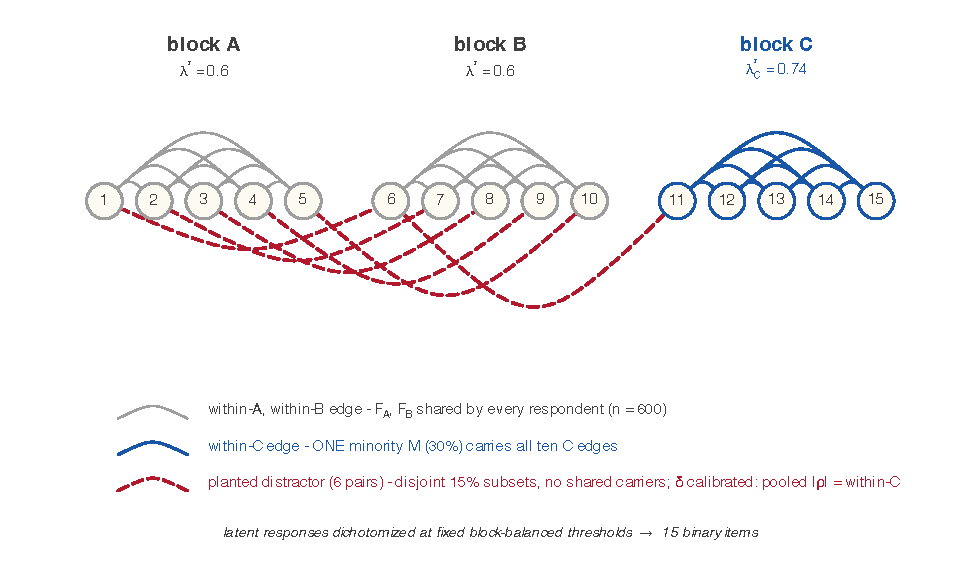
\includegraphics[width=.95\textwidth]{figs/fig_sim1_design.pdf}
\caption{Generative design of the preregistered simulation. Fifteen binary
items in three blocks of five; within-block edges are drawn as arcs above
the item row, the six planted distractor pairs
$(1,6),(2,7),(3,8),(4,9),(5,10),(6,11)$ as dashed arcs below. Blocks A and
B are population-wide: every respondent ($n=600$) shares $F_A$, $F_B$
(standardized loading $\lambda^{*}=.60$). Block C is minority-carried: one
subgroup $M$ ($\pi_C=.30$) carries all ten within-C edges
($\lambda_C^{*}=.74$ within carriers). Each distractor pair receives a
pair-specific factor active only in its own disjoint $15\%$ respondent
subset --- no shared carriers --- with loading $\delta$ calibrated in a
discarded pilot so that mean pooled $|\rho|$ matches the within-C mean.
The design scales the toy contrast of Figure~\ref{fig:toy}: block C
realizes the coherent-minority scenario of panel A, the distractors
realize the disjoint-minorities scenario of panel B, and pooled
correlation cannot separate them.}
\label{fig:simdesign}
\end{figure}
\FloatBarrier  % Figure 2 (design) must precede Section 3.2 (PI 2026-08-26)

\subsection{Two evaluation levels}
The production pipeline first selects candidate edges with the Triangulated
Maximally Filtered Graph (TMFG) on raw
$|\rho|$ \citep{massara2016} --- a standard filtering step that retains a
planar, well-connected subset of the strongest edges and discards the rest
--- and only then reweights retained edges;
carrier weighting cannot rescue an edge TMFG has already removed. The
preregistration therefore mandates two evaluations that may never be
collapsed: an \emph{estimator-level} test on a fixed candidate set
containing all true within-block and distractor edges, and an
\emph{end-to-end} test (raw-$|\rho|$ TMFG $\to$ reweight $\to$ walktrap)
with TMFG availability --- the proportion of the ten true within-C edges retained
--- reported separately. One structural fact sharpens the second level:
the ten within-C edges form the complete graph on the five block-C items
($K_5$), which cannot be drawn in the plane without crossings; since TMFG
returns only planar graphs, it can retain at most nine of the ten
within-C edges. Availability is capped at $.9$ by construction, and the
question is how far below that cap the raw-correlation filter falls.

\subsection{Methods and outcomes}
Four methods --- each usable in practice, since none requires knowing the
true carriers --- receive identical data: raw $|\rho_e|$; the
concentration-only ablation $|\rho_e|(1-G_e)$; the coherence-only ablation
$|\rho_e|\max(\Obar_e,0)$ (an ablation removes one factor of the
estimator, to locate which factor does the work); and the full
carrier-weighted (CW) estimator,
Eq.~\eqref{eq:cw}. The ablations
are mandatory because $(1-G)$ rewards diffuse support and could in
principle penalize the very minority concentration the method aims to
recover. A fifth comparator is an oracle --- it is handed the true carrier
subgroup, information no real analysis could have --- and computes
correlations within that subgroup, serving as a diagnostic only. Estimator-level
outcomes are the area under the receiver operating characteristic curve
(AUROC) for ranking the ten within-C edges above the six
distractors, the mean score separation, and the mechanism check
(distributions of $|\rho|$, $G$, and $\Obar$ from Eq.~\eqref{eq:obar} for
within-C versus distractor edges);
end-to-end outcomes are the adjusted Rand index (ARI; a chance-corrected
agreement between the recovered and true item groupings) against the true
partition, recovery of the correct number of communities ($k{=}3$),
exact recovery of block C, and TMFG availability. All comparisons are
paired by replicate with percentile-bootstrap confidence intervals (CI;
$10{,}000$ resamples).

The preregistration condenses these outcomes into four decision rules,
locked before any confirmatory replicate together with the interpretation
of every pass/fail pattern. Rule~1 is the estimator-level claim: CW must
rank within-C edges above distractors better than raw correlation (AUROC CW $>$
raw). Rule~2 is the end-to-end claim: CW must improve \emph{both} ARI and
exact-C recovery over the raw pipeline. Rule~3 is the specificity control:
in no-structure data, CW must not inflate false $k{=}3$ detections by more
than $.05$ over raw. Rule~4 is the mechanism check: pooled $|\rho|$ must
be matched between within-C edges and distractors (the calibration held), and the
separation, if any, must be carried by $\Obar$ rather than by $G$. Results
are reported below rule by rule.

\subsection{Results}\label{sec:results}
Rule~1 passed: AUROC $.985$ for CW versus $.469$ for raw, a
paired-bootstrap difference of $+.516$ with $95\%$ CI $[+.506,+.526]$;
the companion outcome, mean score separation (mean weight of within-C
edges minus distractors), was $+.013$ for CW versus $-.007$ for raw.
Rule~2 \emph{failed}: the ARI difference $+.0034$ $[+.0001,+.0067]$
excludes zero, but the exact-C difference $+.0020$ $[-.0080,+.0120]$
does not. Rule~3 passed: false $k{=}3$ rates were $.295$ (raw) and
$.308$ (CW), a difference of $+.013$. The absolute rates warrant a
comment the rule itself does not require: with the C loadings set to
zero, the six distractor pairs remain in the data, and the
candidate-selection and community-detection stages shared by both
pipelines assemble a spurious third community in roughly $30\%$ of null
replicates. That rate is a property of TMFG-plus-walktrap on null data,
essentially unchanged by reweighting; the rule targets the increment,
which is the only quantity the estimator could affect. Rule~4 passed: pooled $|\rho|$ was
matched (C $.169$, distractor $.176$), Gini did \emph{not} separate the
classes ($.172$ / $.165$), and $\Obar$ did ($.102$ / $-.003$).

Rule 4 is the wedge argument of Section~\ref{sec:wedge} confirmed at scale
(Figure~\ref{fig:mechanism}): with pooled magnitude matched by design,
concentration is indistinguishable between real minority edges and
distractors --- the concentration-only ablation achieves AUROC $.464$,
chance --- while coherence separates them cleanly, and coherence-only
($.985$) matches the full estimator (Figure~\ref{fig:ablation}). The
oracle comparator returned an
\emph{inverted} AUROC of $.002$: within-carrier correlation is higher for
distractor cliques than for within-C edges at the calibrated $\delta$, because
both mechanisms are perfectly real within their own carriers. Only
cross-edge coherence distinguishes them --- which is the thesis, so the
oracle is reported as a diagnostic, not a competitor.

\begin{figure}[!htb]
\centering
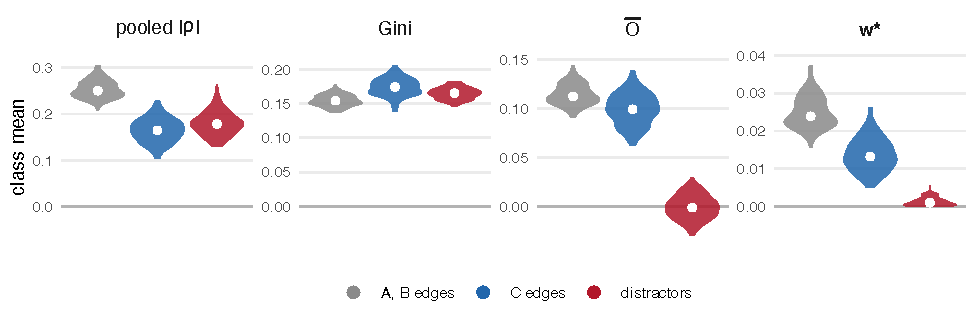
\includegraphics[width=.9\textwidth]{figs/fig2_mechanism.pdf}
\caption{Mechanism check, all 36 structural edge classes (per-replicate
class means over the 100 archived per-edge replicates; C and distractor
values agree with the 1{,}000-replicate summary statistics). Pooled
$|\rho|$ is matched between minority-carried within-C edges and incoherent
distractors by calibrated design, with both below the population-wide A/B
level; Gini concentration separates none of the three classes;
the coherence statistic $\Obar$ alone isolates the distractors, while
population-wide A/B edges and minority-carried within-C edges are both coherent.
The resulting weight $\wstar$ (rightmost panel) preserves the A/B and
within-C edges and drives the distractors to near zero: survival is decided by the
coherence gate, not by magnitude or concentration. Class separability is
quantified by the edge-level AUROC values reported in the text, not by
significance tests on replicate means, whose $p$-values would reflect
only the number of simulation replicates.}
\label{fig:mechanism}
\end{figure}

\begin{figure}[t]
\centering
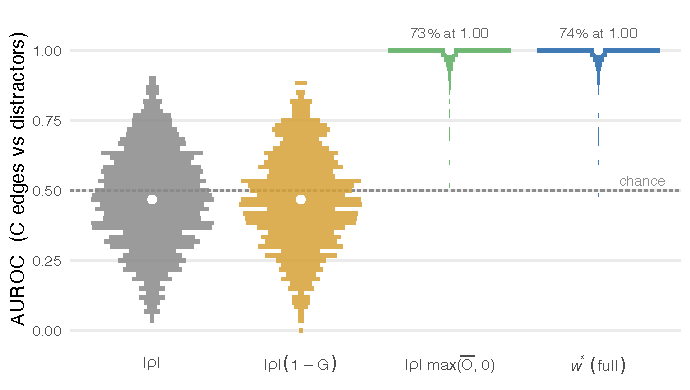
\includegraphics[width=.72\textwidth]{figs/fig4_ablation.pdf}
\caption{Ablation, estimator-level AUROC (within-C edges versus distractors) over
1{,}000 replicates; axis labels give each arm's scoring formula. AUROC
over the $10\times6$ C--distractor pairs is discrete (grid $1/60$), so
each horizontal bar marks one attained value, with bar width
proportional to the number of replicates at that value (normalized
within arm); white dots mark medians. The concentration-only
ablation $|\rho|(1-G)$ is at chance (mean $.464$); the coherence-only
ablation $|\rho|\max(\Obar,0)$ carries the effect ($.985$); the full
$\wstar$ matches it ($.985$) --- the a-priori prediction of
Section~\ref{sec:wedge}. The right-hand distributions collapse onto a
single dominant bar at ceiling (73--74\% of replicates at AUROC exactly
$1.00$, annotated) with a short tail below. The oracle subgroup comparator (mean AUROC
$.002$, inverted) is reported in the text as a diagnostic.}
\label{fig:ablation}
\end{figure}

\FloatBarrier  % Figures 3-4 must precede the end-to-end/failure-map passage (PI 2026-08-26)

The end-to-end level tells a different and equally preregistered story.
At $n=600$ and $\pi_C=.30$ the raw pipeline already recovers the
partition well, leaving little headroom: the per-replicate ARI
distributions of the two pipelines nearly coincide (mean $.946$ raw
versus $.949$ CW), and exact-C recovery is likewise indistinguishable
($.815$ versus $.817$; paired difference $+.0020$, CI spanning zero as
reported above), and recovery of the correct number of communities was
near ceiling in both arms ($.987$ raw, $.973$ CW). These results provide no evidence of an end-to-end
improvement. Exact-C recovery depended strongly on the availability of true
within-C edges in the shared raw-$|\rho|$ TMFG. When the graph retained the structural
maximum of nine of the ten possible within-C edges, exact recovery was nearly
certain ($.99$); below that maximum, it fell to $.37$ and was essentially the
same for raw and CW. Because both arms used the same candidate graph, CW could
reweight retained edges but could not restore edges removed by TMFG. The
preregistered comparison therefore tests carrier-aware reweighting after raw-
correlation edge selection, not carrier-aware edge selection itself.

The preregistered secondary analyses --- the $36$-condition parameter grid
(generalization analyses) and bootstrap stability outcomes --- have not yet
been completed and are not
reported here. The present report is limited to the primary condition; those
secondary results will be reported separately.
% PI DECISION 2-3 resolved 2026-08-27: grid + bootstrap deferred, wording
% changed to "were not executed" (external review flagged ambiguity).

% =============================================================================
\section{Empirical illustration}\label{sec:empirical}
The estimator originated in a concrete measurement problem: the
Gray--Wheelwright Jungian Type Survey, whose thinking--feeling axis is the
least well established of its three --- coefficient alpha $.38$, against
$.72$ for introversion--extraversion and $.70$ for intuition--sensation
\citep{davis2006,mattoon1995}.
This is the situation the estimator targets. If part of an axis is
carried coherently by a minority of respondents, its pooled correlations
are diluted toward the magnitude of incidental associations, and a
candidate graph built on pooled correlation alone cannot tell the two
apart (Section~\ref{sec:wedge}).

In the companion application that motivated this paper ($n=605$
respondents to the 81-item Korean form, tetrachoric correlations, TMFG
candidate graph, walktrap community detection), Eq.~\eqref{eq:cw}
replaced the raw edge weights inside an otherwise unchanged bootEGA
pipeline. Its role there is exactly the estimator-level role
validated in Section~\ref{sec:sim}: an item-pair association that
appears in the group average but is not carried by the respondents who
carry its neighbouring edges is down-weighted before community detection
and bootstrap stability assessment, so that item-retention decisions
rest on coherently carried structure rather than on aggregation
artefacts. Substantive results on the instrument --- item selection, the
refined forms, and their reliability --- are reported in a separate
manuscript (in submission) and are not claimed here; the illustration
shows that the estimator's target phenomenon arises in real psychometric
data and that the estimator deploys there without any modification of
the surrounding pipeline.

% =============================================================================
\section{Discussion}\label{sec:discussion}
What the simulation establishes is deliberately narrow and, within that
scope, unambiguous. At the estimator level, carrier coherence separates
minority-carried structure from matched incoherent distractors at AUROC
$.985$, with $73$--$74\%$ of replicates at exactly $1.00$; the mechanism
operates exactly as the wedge argument predicts,
and the separation is attributable to the coherence factor alone: the
concentration-only ablation sits at chance. What the simulation does \emph{not}
establish is an end-to-end recovery advantage at $n=600$ --- Rule~2 failed,
and the paper claims edge-level separation, not end-to-end recovery, for
that reason. Rule~2 compared pipelines that shared one candidate graph,
selected by raw correlation; it therefore tested reweighting, not
selection.

The ablation result also disciplines the formula itself. The
coherence-only ablation performed indistinguishably from the full
estimator. Because the formula was locked, this licenses discussion of the
$(1-G)$ factor's role --- not its post-hoc revision --- and the honest
reading is sharper than ``neither helps nor harms.'' Analytically, $G$
depends only on the magnitudes $|S_{re}|$, never on their signs, and is
therefore direction-blind: toy scenarios A and B have identical $G$ by
construction, so the factor cannot contribute to detection. Concentration of support is,
moreover, the mathematical signature of \emph{any} minority-carried edge,
coherent or spurious, and the concentration information that matters in the
network context is already accounted for by $\Obar$, conditionally on
alignment: misaligned concentration depresses the carrier cosines through
their normalization, while aligned concentration is precisely the signal. What
$(1-G)$ adds beyond $\Obar$ is an \emph{unconditional} penalty on
minority-ness itself, in direct tension with the estimator's motivation. A
deterministic dilution sequence makes the tension concrete
(Table~\ref{tab:dilution}). It is computed exactly by hand from the toy
construction, hence not tuned on confirmatory data: the three-carrier
scenario-A structure is held fixed while the all-zero background grows.
Both evidence terms ($|\rho|$ and $\Obar$) strengthen monotonically, yet
the full weight $\wstar$ is non-monotone and lowest exactly where the
evidence is strongest, with $\wstar\to0$ as the coherent minority becomes
rarer --- the paper's own headline use-case. Nor
does $(1-G)$ serve as an uncertainty proxy: it depends on the carried
\emph{fraction} of the sample, whereas sampling precision scales with the
absolute \emph{number} of carrying respondents, an inferential question
that belongs to resampling downstream, not to the point estimator. Equation~\eqref{eq:cw} retains
$(1-G)$ because the preregistration locked it; retention is
preregistration discipline, not endorsement. Whether a Gini-free variant,
or one weighted by the effective number of carriers rather than their
fraction, should replace it is the subject of the next preregistration;
concentration would in any case remain reported per edge, as an annotation
giving carrier count and carrier share alongside the weight. The preregistration's own
interpretation table anticipated exactly this contingency.

\begin{table}[!htb]
\centering
\caption{Deterministic dilution of the scenario-A triangle: the three
carriers are held fixed while the all-zero background grows. Every value
is an exact hand computation from the toy construction (no simulation,
no tuning). Both evidence terms strengthen monotonically; the $(1-G)$
factor drives the full CW weight down exactly where the evidence is
strongest, while the Gini-free product $|\rho|\max(\Obar,0)$ is monotone
in the evidence.}
\label{tab:dilution}
\begin{tabular}{lccccc}
\toprule
carriers & $\rho$ & $\Obar$ & $1-G$ &
$\wstar$ (CW) & $|\rho|\max(\Obar,0)$\\
\midrule
3/18 (16.7\%)  & .397 & $+.667$ & .712 & .188 & .265\\
3/36 (8.3\%)   & .651 & $+.947$ & .379 & .234 & .617\\
3/60 (5.0\%)   & .737 & $+.985$ & .234 & .170 & .726\\
3/120 (2.5\%)  & .804 & $+.997$ & .121 & .097 & .802\\
\bottomrule
\end{tabular}
\end{table}

Three limitations bound the claims. First, when two carrier subgroups
couple the same item pair with opposite signs in equal measure, the pooled
correlation itself cancels toward zero, and no reweighting of a near-zero
edge can rescue it; a coherence statistic that tracks positive and
negative alignment separately is future work. Second, the method addresses
between-respondent heterogeneity in cross-sectional data and says nothing
about within-person dynamics. Third --- and most consequentially --- the
end-to-end analysis shows that the current pipeline's bottleneck is upstream
of the estimator: raw-correlation TMFG can discard true minority-carried edges
that no subsequent reweighting can recover. Carrier-aware candidate-edge
selection therefore requires a new, independently preregistered study.
Companion work
extending the carrier construction to directed, flow-like associations and
to permutation-based inference is developed elsewhere.

% =============================================================================
\section*{Reproducibility statement}
The preregistration and its pre-confirmatory amendment are archived,
date-stamped, in the project repository alongside the engine
(\texttt{sim1\_engine.R}), the analysis and figure scripts, and an md5
manifest of all outputs. All seeds are published (calibration 20260718,
discarded; confirmatory 202608250001--202608251000; control
202608260001--202608261000), and the deterministic map from nominal seed
IDs to random-number-generator seeds is documented in the engine. The confirmatory run used
R~4.5.1 with \texttt{psych}~2.6.5, \texttt{NetworkToolbox}~1.4.4, and
\texttt{igraph}; figures were produced by a single script from the archived
outputs. The repository is public at
\url{https://github.com/ad0c1/CW_unified}.

\bibliographystyle{plainnat}
\begin{thebibliography}{10}

\bibitem[Christensen and Golino(2021)]{christensen2021}
Christensen, A.~P., and Golino, H. (2021).
Estimating the stability of psychological dimensions via bootstrap
exploratory graph analysis: A Monte Carlo simulation and tutorial.
\emph{Psych}, 3(3), 479--500.

\bibitem[Davis and Mattoon(2006)]{davis2006}
Davis, M.~F., and Mattoon, M.~A. (2006).
Reliability and validity of the Gray-Wheelwrights Jungian Type Survey.
\emph{European Journal of Psychological Assessment}, 22(4), 233--239.

\bibitem[Epskamp and Fried(2018)]{epskamp2018}
Epskamp, S., and Fried, E.~I. (2018).
A tutorial on regularized partial correlation networks.
\emph{Psychological Methods}, 23(4), 617--634.

\bibitem[Fisher et~al.(2018)]{fisher2018}
Fisher, A.~J., Medaglia, J.~D., and Jeronimus, B.~F. (2018).
Lack of group-to-individual generalizability is a threat to human subjects
research. \emph{Proceedings of the National Academy of Sciences}, 115(27),
E6106--E6115.

\bibitem[Golino and Epskamp(2017)]{golino2017}
Golino, H.~F., and Epskamp, S. (2017).
Exploratory graph analysis: A new approach for estimating the number of
dimensions in psychological research. \emph{PLoS ONE}, 12(6), e0174035.

\bibitem[Jamison et~al.(2024)]{jamison2024}
Jamison, L., Christensen, A.~P., and Golino, H.~F. (2024).
Metric invariance in exploratory graph analysis via permutation testing.
\emph{Methodology}, 20(2), e12877.

\bibitem[Massara et~al.(2017)]{massara2016}
Massara, G.~P., Di~Matteo, T., and Aste, T. (2017).
Network filtering for big data: Triangulated maximally filtered graph.
\emph{Journal of Complex Networks}, 5(2), 161--178.

\bibitem[Mattoon and Davis(1995)]{mattoon1995}
Mattoon, M.~A., and Davis, M. (1995).
The Gray-Wheelwrights Jungian Type Survey: Development and history.
\emph{Journal of Analytical Psychology}, 40(2), 205--234.

\bibitem[Molenaar(2004)]{molenaar2004}
Molenaar, P.~C.~M. (2004).
A manifesto on psychology as idiographic science: Bringing the person back
into scientific psychology, this time forever. \emph{Measurement:
Interdisciplinary Research and Perspectives}, 2(4), 201--218.

\bibitem[Pons and Latapy(2006)]{pons2006}
Pons, P., and Latapy, M. (2006).
Computing communities in large networks using random walks.
\emph{Journal of Graph Algorithms and Applications}, 10(2), 191--218.

\end{thebibliography}

\appendix
\section{Preregistration deviations}\label{app:deviations}
One amendment, made before any confirmatory replicate was run and
authorized by the preregistration's revision rule (``any revision creates
Simulation 1b with a new file, seeds, and decision rules''):

\begin{center}
\begin{tabular}{@{}llll@{}}
\toprule
Parameter & Preregistered & Amended (1b) & Reason \\
\midrule
Pair factor $D_{r,d}$ & $N(0,1)$ & $N(1,1)$ &
  \begin{tabular}[t]{@{}l@{}}zero-mean factor saturates under\\
  dichotomization (concordant-1 cell\\ capped at $\pi_D/2$)\end{tabular} \\
\addlinespace
Distractor prevalence $\pi_D$ & $.10$ & $.15$ &
  \begin{tabular}[t]{@{}l@{}}calibration target unreachable at\\
  $.10$ for any $\delta$ ($\delta$-grid evidence\\ archived in
  amendment file)\end{tabular} \\
\addlinespace
Confirmatory seed block & 2026071800xx & 2026082500xx &
  original block retired unused \\
\bottomrule
\end{tabular}
\end{center}

The calibration target, decision rules, and all other parameters are
unchanged. The original seed block was never executed; the amendment file
records the full $\delta$-grid from the discarded pilot.

\end{document}
